\documentclass[a4paper,11pt,cours]{nsi} % COMPILE WITH DRAFT
\geometry{margin=2cm}
\usepackage[]{fontawesome5}

\setcounter{chapter}{1} % 1 de moins que le num de chapitre

\setlength{\columnseprule}{0.5pt}
\setlength{\columnsep}{1cm}

\chapter{Fonctions : limites et continuité}

\begin{document}

\section{Rappels sur la dérivation}
\subsection*{Dérivées des fonctions de référence}
\begin{propriete}[ ]
	On note $D_f$ l'ensemble de définition de la fonction $f$ et $D_{f'}$ son ensemble de dérivabilité.\\
	
	\renewcommand{\arraystretch}{2}
	\begin{tabular}{|c|c|c|c|}
		\hline
		\textbf{Fonction $f$ définie par :} & $D_f$ & \textbf{Fonction dérivée $f'$ définie par :} & $D_{f'}$\\
		\hline
		
		$f(x)=k$, avec $k\in \R$ & $\R$ & $f'(x)=0$ & $\R$ \\
		\hline
		$f(x)=mx+p$, avec $m,p \in \R$ & $\R$ & $f'(x)=m$ & $\R$ \\
		\hline
		$f(x)=x^2$ & $\R$ & $f'(x)=2x$ & $\R$ \\
		\hline
		$f(x)=x^n$, avec $n\in \N^*$ & $\R$ & $f'(x)=nx^{n-1}$ & $\R$ \\
		\hline
		$f(x)=\dfrac{1}{x}$ & $\R \backslash \{0\}$ & $f'(x)=-\dfrac{1}{x^2}$ & $\R\backslash \{0\}$ \\
		\hline
		$f(x)=\dfrac{1}{x^n}$, avec $n\in \N^* $& $\R \backslash \{0\}$ & $f'(x)=-\dfrac{n}{x^{n+1}}$ & $\R\backslash \{0\}$ \\
		\hline
		$f(x)=\sqrt{x}$ & $\fio{0}{+\infty}$ & $f'(x)=\dfrac{1}{2\sqrt{x}}$ & $\oio{0}{+\infty}$\\
		\hline
	\end{tabular}
\end{propriete}


\newpage
\subsection*{Fonctions dérivées et opérations}
\begin{propriete}[]
    Soient $u$ et $v$ deux fonctions définies et dérivables sur un même intervalle ouvert $I$ et $k$ un nombre réel.
    \begin{enumerate}[label=\textbullet]
        \item La fonction $u+v$ est dérivable sur $I$ et $\quad (u+v)'=u'+v'$.
        \item La fonction $ku$ est dérivable sur $I$ et $\quad (ku)'=ku'$.
\newpage
        \item La fonction $u\times v$ est dérivable sur $I$ et $\quad (u\times v)'=u'v+ uv'$.
        \item Si, pour tout $x\in I, v(x)\neq 0$, alors :
        \begin{itemize}
            \item la fonction $\dfrac{1}{v}$ est dérivable sur $I$ et $\quad \left(\dfrac{1}{v}\right)'=-\dfrac{v'}{v^2}$.
            \item la fonction $\dfrac{u}{v}$ est dérivable sur $I$ et $\quad \left(\dfrac{u}{v}\right)'=\dfrac{u'v-uv'}{v^2}$.
        \end{itemize}
	\end{enumerate}
\end{propriete}

\begin{propriete}[]
	Soit $g$ une fonction définie et dérivable sur un intervalle $I$.\\
	Soient $a$ et $b$ deux réels et soit $J$ l'intervalle tel que pour tout $x\in J, ax+b \in I$.\\[.5em]
	La fonction $f:x\mapsto g(ax+b)$ est définie et dérivable sur $J$ et
		$\quad f'(x)=a\times g'(ax+b)$.
\end{propriete}

\subsection*{Sens de variation, extremum local et dérivée}

\begin{propriete}[]
	Soit $f$ une fonction dérivable sur un intervalle $I$.
	\begin{enumerate}[label=\textbullet]
		\item Si, pour tout réel $x$ de $I$, $f'(x)>0$ (sauf éventuellement en un nombre fini de point où elle s'annule), alors la fonction $f$ est \textbf{strictement croissante} sur $I$.
		\item Si, pour tout réel $x$ de $I$, $f'(x)<0$ (sauf éventuellement en un nombre fini de point où elle s'annule), alors la fonction $f$ est \textbf{strictement décroissante} sur $I$.
	\end{enumerate}
\end{propriete}

\begin{propriete}[]
	Soient $f$ une fonction dérivable sur un intervalle ouvert $i$ et $c$ un réel appartenant à $I$.\\
	Si $f'$ \textbf{s'annule et change de signe} en $c$, alors $f(c)$ est un \textbf{extremum local} de $f$.
\end{propriete}



\begin{exemple}[s]
	On considère une fonction $f$ définie sur un intervalle $\oio{a}{b}$ contenant $c$.
	\begin{multicols}{2}
		\begin{center}
			\begin{tikzpicture}
			\tkzTabInit[color,lgt=2,espcl=2]
			{$x$/.7,$f'(x)$ /.7,$f$ /1.4}
			{$a$,$c$, $b$}
			\tkzTabLine{,-,z,+,}
			\tkzTabVar{+/,-/$f(c)$,+/}
			\end{tikzpicture}
			\end{center}
			$f(c)$ est un minimum local.\\
		\begin{center}
			\begin{tikzpicture}
			\tkzTabInit[color,lgt=2,espcl=2]
			{$x$/.7,$f'(x)$ /.7,$f$ /1.4}
			{$a$,$c$, $b$}
			\tkzTabLine{,+,z,-,}
			\tkzTabVar{-/,+/$f(c)$,-/}
			\end{tikzpicture}
			\end{center}
			$f(c)$ est un maximum local.\\	
	\end{multicols}
\end{exemple}

\section{La fonction exponentielle}

\subsection*{Définition de la fonction exponentielle}
\begin{propriete}[]
	Il existe une unique fonction $f$ définie et dérivable sur $\R$ vérifiant : 
	$$\text{pour tout nombre réel }x  \quad f'(x)=f(x)\quad \text{et} \quad f(0)=1.$$
\end{propriete}
%\begin{demonstration}
%	L'existence de cette fonction est admise.\\
%	La démonstration de l'unicité pourra être faite en exercice.
%\end{demonstration}

\begin{definition}[ ]
	La \textbf{fonction exponentielle} est la fonction, notée $\exp$, définie et dérivable sur $\R$ telle que $\exp(0)=1 \ $ et $\ \exp'=\exp$.
\end{definition}

%\begin{methode}[ ]
%	\textbf{Déterminer la fonction $f$ définie et dérivable sur $\R$ telle que $f'=f$ et $f(0)=3$.}\\
%	On pose : pour tout $x\in \R, f(x)=3\exp(x)$.\\
%	Cette égalité définit la fonction $f$ qui est bien définie et dérivable sur $\R$.\\
%	Pour $x\in \R, \quad f'(x)=3\exp'(x)=3\exp(x)=f(x)$.
%\end{methode}


\subsection*{Propriétés algébriques}
\begin{propriete}[ ]
	La fonction exponentielle est \textbf{strictement positive} : $\quad \text{pour tout } x\in \R,\ \exp(x)>0$.
\end{propriete}
%\newpage


%\begin{demonstration}
%	La démonstration pourra être faite en exercice.
%\end{demonstration}

\begin{propriete}[ : Relation fonctionnelle]
	Pour tous nombres réels $x$ et $y$, $\quad \boxed{\exp(x+y)=\exp(x)\times \exp(y)}$.
\end{propriete}
\begin{demonstration}
	Soit $y$ un nombre réel fixé.\\
	On définit la fonction $f$ par : pour tout $x\in \R$, $\ f(x)=\dfrac{\exp(x+y)}{\exp(x)}$.\\
	$f$ est dérivable sur $\R$ comme quotient de fonctions dérivables sur $\R$ et, pour tout réel $x$, $$f'(x)=\dfrac{\exp(x+y)\exp(x)-\exp(x+y)\exp(x)}{\left[\exp(x)\right]^2}=0$$
	On en déduit que $f$ est une fonction \textbf{constante}. Ainsi, pour tout $x\in \R, \ f(x)=f(0)=\exp(y)$.\\
	On a donc montré que $\dfrac{\exp(x+y)}{\exp(x)}=\exp(y)$. Ainsi $\exp(x+y)=\exp(x)\times\exp(y)$.
\end{demonstration}

\begin{propriete}[ ]
	Pour tout nombre réel $x$, $\quad \exp(x)\times \exp(-x)=1 \quad$ et $\quad \exp(-x)=\dfrac{1}{\exp(x)}$.
\end{propriete}
\begin{demonstration}
	Soit $x$ un nombre réel. 
	On applique le théorème précédent à $x$ et $-x$. On obtient :
	\begin{tabbing}
		$\exp(x)\times \exp(-x)$ \= $=\exp(x-x)$\\
		\>	$=\exp(0)$\\
		\>	$=1$
	\end{tabbing}
	Ainsi, pour tout $x\in \R$, $\exp(x)$ et $\exp(-x)$ sont inverses l'un de l'autre. Donc $\exp(-x)=\dfrac{1}{\exp(x)}$.
\end{demonstration}

\begin{propriete}[]
	Pour tous nombres réels $x$ et $y$, $\quad\exp(x-y)=\dfrac{\exp(x)}{\exp(y)}$.
\end{propriete}
%\newpage


%\begin{demonstration}
%	En exercice
%\end{demonstration}

\begin{propriete}[ (admise)]
	Pour tout réel $x$ et tout entier relatif $n$, $\quad \boxed{\left[\exp(x)\right]^n=\exp(nx)}$.
\end{propriete}

\setlength{\columnseprule}{0pt}

\begin{exemple}[s]
\begin{multicols}{3}
	\begin{enumerate}[label=\textbullet]
		\item 	\begin{tabbing}
			$\exp(3)\times\exp(7)$	\= $=\exp(3+7)$\\
			\>	$=\exp(10)$
		\end{tabbing}
		\item 	$\exp(-5)=\dfrac{1}{\exp(5)}$
		\item	\begin{tabbing}
			$\left(\exp(2)\right)^4$	\= $=\exp(4\times 2)$\\
			\>	$=\exp(8)$
		\end{tabbing}
	\end{enumerate}	
\end{multicols}
\end{exemple}

%\begin{exercice}[]
%	Simplifier les expressions suivantes :
%	\begin{multicols}{2}
%		\begin{enumerate}[]
%			\item 	$\exp(5)\times \exp(8) \times \left[\exp(2)\right]^3$\\[0.5em]
%			\carreauxseyes{7.2}{3.2}
%			\item 	$\exp(5)\times \left(\exp(5)\right)^{-1}\times\exp(10)$\\[0.5em]
%			\carreauxseyes{7.2}{3.2}
%		\end{enumerate}
%	\end{multicols}
%\end{exercice}

\subsection*{Le nombre $e$}
\begin{definition}[ ]
	On note $\quad \exp(1)=e$
\end{definition}

\begin{remarque}[s]
	\begin{enumerate}[label=\textbullet]
		\item 	$e$ est un nombre réel irrationnel.
		\item 	$e \approx 2,718$
		\item	Pour tout $n\in\N, \quad \exp(n)=\exp(n\times 1)=\left[\exp(1)\right]^n=e^n$.	
	\end{enumerate}
\end{remarque}
	
\begin{notation}[ ]
	Par extension, pour tout $x\in \R$, on notera : $\quad \exp(x)=e^x$.
\end{notation}

\setlength{\columnseprule}{0pt}
\setlength{\columnsep}{0.5cm}

\begin{propriete}[]
	Avec cette notation, les propriétés vues précédemment s'écrivent :\\
	Pour tous $x, y$ réels et tout $n$ entier relatif,
	\begin{multicols}{5}
		\begin{enumerate}[label=\textbullet]
			\item 	$e^{x+y}=e^x\times e^y$
			\item 	$e^x\times e^{-x}=1$
			\item	$e^{-x}=\dfrac{1}{e^x}$
			\item	$e^{x-y}=\dfrac{e^x}{e^y}$
			\item	$\left(e^x\right)^n=e^{nx}$
		\end{enumerate}
	\end{multicols} 
\end{propriete}

\begin{exemple}[]
	\begin{tabbing}
		$\dfrac{\left(e^7\right)^4\times e^3}{e^4}$	\= $=\dfrac{e^{7\times 4}\times e^3}{e^4}$\\[0.5em]
		\>	$=\dfrac{e^{28}\times e^3}{e^4}$\\[0.5em]
		\>	$=e^{28+3-4}$\\[0.5em]
		\>	$=e^{27}$
	\end{tabbing}
\end{exemple}

\subsection*{Variations de la fonction exponentielle}

\begin{propriete}[]
	La fonction exponentielle est strictement croissante sur $\R$.
	\begin{center}
		\def\xmin{-5} \def\ymin{-1}\def\xmax{3}\def\ymax{5}
		\def\F{exp(\x)}
		\begin{tikzpicture}[scale=.8]
			\clip (\xmin,\ymin) rectangle (\xmax,\ymax);
			\draw[fill = white] (\xmin,\ymin) rectangle (\xmax,\ymax);
			\repereal{\xmin}{\ymin}{\xmax}{\ymax}
			\draw[color=UGLiOrange,thick,domain=\xmin:3,smooth,variable=\x] plot ({\x},{\F});
			\draw[color=UGLiOrange] (2,4.5) node{\courbe{\exp}};
			\draw[color=olive] (4,4) node{(T)};
			\draw[color=olive,thick,domain=\xmin:\xmax,smooth,variable=\x] plot ({\x},{\x+1});
			\pointc{1}{2.718}{}{$e$}{$A$}
			
		\end{tikzpicture}
	\end{center}
\end{propriete}
%\newpage


\begin{demonstration}
	Pour tout $x\in\R, \exp'(x)=\exp(x)>0$.\\
	la fonction dérivée de la la fonction exponentielle est strictement positive sur $\R$ donc la fonction exponentielle est strictement croissante sur $\R$.
\end{demonstration}

\begin{propriete}[ ]
	Soient $a$ et $b$ deux nombres réels. On définit la fonction $f$ sur $\R$ par $\quad f(x)=e^{ax+b}$.\\
	La fonction $f$ est dérivable sur $\R$ et pour tout $x\in \R, \quad f'(x)=a\ e^{ax+b}$.
\end{propriete}
\begin{demonstration}
	Soient $a$ et $b$ deux nombres réels.\\
	La dérivée de $f$ définie par $f(x)=g(ax+b)$ était donnée par : $\quad f'(x)=a\ g'(ax+b)$.\\
	On applique cette propriété avec $g=\exp$ et on obtient le résultat.
\end{demonstration}

\begin{exemple}[ ]
	\textbf{\'Etude des variations d'une fonction :}\\
	La fonction $h$ définie sur $\R$ par $\quad h(x)=-3\ e^{2x-5}+1\quad$ est dérivable sur $\R$ et pour tout $x\in\R$,
	\begin{tabbing}
		$h'(x)$	\= $=2\times \left(-3\ e^{2x-5}\right)+0$\\
		\>	$=-6\ e^{2x-5}$
	\end{tabbing}
	Pour tout $x\in\R, \quad e^{2x-5}>0,\quad$ donc $h'(x)<0$.\\
	La fonction $h$ est donc strictement décroissante sur $\R$.
\end{exemple}

\subsection*{Applications : résolutions d'équations et d'inéquations}

\begin{propriete}[s]
Pour tous nombres réels $a$ et $b$ :
\begin{multicols}{2}
	\begin{enumerate}[label=\textbullet]
		\item 	$e^{a}=e^{b}\ \Leftrightarrow\ a=b$
		\item 	$e^{a}<e^{b}\ \Leftrightarrow\ a<b$
	\end{enumerate}
\end{multicols}
\end{propriete}

\begin{exemple}[s]
	\begin{multicols}{2}
		\begin{enumerate}[label=\textbullet]
			\item 	\textbf{Résolution d'équation :}\\
			Résoudre dans $\R \quad e^{2x}=\dfrac{1}{e}$ \\
			Soit $x\in\R$
			\begin{tabbing}
				$e^{2x}=\dfrac{1}{e} \quad$		\=	$\Leftrightarrow\quad e^{2x}=e^{-1}$\\
				
				\>	$\Leftrightarrow\quad 2x=-1$\\
				\>	$\Leftrightarrow \quad x=-\dfrac{1}{2}$
			\end{tabbing}
			L'équation $e^{2x}=\dfrac{1}{e}$ a pour unique solution $-\dfrac{1}{2}$.
			\vspace{0.8cm}
			\item	\textbf{Résolution d'inéquation :}\\
			Résoudre dans $\R \quad e^{-3x+4}+1\geqslant2$.\\
			Soit $x\in\R$.
			\begin{tabbing}
				$e^{-3x+4}+1\geqslant2 \quad$		\=	$\Leftrightarrow\quad e^{-3x+4}\geqslant1$\\
				
				\>	$\Leftrightarrow\quad  e^{-3x+4}\geqslant e^{0}$\\
				
				\> $\Leftrightarrow\quad -3x+4\geqslant 0$\\
				
				\> $\Leftrightarrow\quad x\leqslant\dfrac{4}{3}$
			\end{tabbing}
			L'ensemble des solutions de l'inéquation $e^{-3x+4}+1\geqslant2$ est l'intervalle $\oif{-\infty}{\dfrac{4}{3}}$.
		\end{enumerate}
	\end{multicols}
	
	
\end{exemple}
%\newpage
\begin{aretenir}
\includegraphics[width=14.7cm]{cartementale}
\end{aretenir}



\section{Limite d'une fonction en l'infini}
Dans cette partie, on considère une fonction $f$ définie sur l'intervalle considéré. La courbe représentative de $f$ est notée $\mathcal{C}_f$ et $n$ désigne un entier naturel non nul.

\begin{definition}[ : Limite infinie]
	\dleft{10cm}{
			On dit que la fonction $f$ a pour \textbf{limite $+\infty$ en $+\infty$} lorsque tout intervalle $\oio{M}{+\infty}$ contient toutes les valeurs de $f(x)$ pour $x$ suffisamment grand (c'est à dire lorsque $x$ appartient à un intervalle $\oio{A}{+\infty}$). On note alors :
	$$\lim\limits_{x\to+\infty}f(x)=+\infty$$
	}
	{
		\begin{center}
			\includegraphics[width=5cm]{limite2.jpg}
		\end{center}
	}
	
\end{definition}

\begin{remarque}[]
	On définit de façon analogue : $\quad \lim\limits_{x\to+\infty}f(x)=-\infty\ ; \quad \lim\limits_{x\to-\infty}f(x)=+\infty\ ; \quad \lim\limits_{x\to-\infty}f(x)=-\infty$.
\end{remarque}


\begin{definition}[s : Limite finie et asymptote horizontale]
	Soit $\ell$ un nombre réel.\\[.5em]
	\dleft{10cm}{
		On dit que la fonction $f$ a pour \textbf{limite $\ell$ en $+\infty$}  lorsque tout intervalle ouvert contenant $\ell$ contient toutes les valeurs de $f(x)$ pour $x$ suffisamment grand (c'est à dire lorsque $x$ appartient à un intervalle $\oio{A}{+\infty}$). On note alors :
		$$\lim\limits_{x\to +\infty} f(x)=\ell$$
		La droite $\Delta$ d'équation $y=\ell$ est alors \textbf{asymptote horizontale} à la courbe $\mathcal{C}_f$.
	}
	{
		\begin{center}
			\includegraphics[width=5cm]{limite1.jpg}
		\end{center}
	}
\end{definition}

\begin{remarque}[]
	On définit de façon analogue : $\quad \lim\limits_{x\to-\infty}f(x)=\ell$.
\end{remarque}


\begin{propriete}[ : limites des fonctions usuelles]
	\tabstyle[UGLiRed]
    \begin{tabular}{|c|c|c|p{2.1cm}|p{1.75cm}|c|p{1.7cm}|c|c|c|p{1.75cm}|}
    \hline
    \ccell $f(x)$ & $x^2$ & $x^3$ & \centering{$x^n$} & \centering{$\sqrt{x}$} &$e^x$ & \centering{$e^{ax}$} &$\dfrac{1}{x}$ & $\dfrac{1}{x^2}$ & $\dfrac{1}{x^n}$ & $\quad \dfrac{1}{\sqrt{x}}$ \\\hline
    
	\ccell $\lim\limits_{x\to+\infty} f(x)$ & $+\infty$ &$+\infty$ & \centering{$+\infty$} & \centering{$+\infty$} & $+\infty$  & \footnotesize{$+\infty$ si $a>0$ $0$ si $a<0$} & $0$ & $0$ & $0$ & $\qquad 0$ \\\hline
    
	\ccell $\lim\limits_{x\to-\infty} f(x)$ & $+\infty$ & $-\infty$  & \footnotesize{$+\infty$ si $n$ pair $-\infty$ si $n$ impair} & \footnotesize{non définie sur $\oio{-\infty}{0}$} & $0$ & \footnotesize{$0$ si $a>0$ $-\infty$ si $a<0$} & $0$ & $0$ & $0$ & \footnotesize{non définie sur $\oif{-\infty}{0}$} \\\hline
    \end{tabular}
\end{propriete}


\section{Limite d'une fonction en un nombre réel}

Dans cette partie, on considère une fonction $f$ définie sur l'intervalle considéré. Le nombre réel $a$ appartient ou est une borne de l'ensemble de définition de $f$. La courbe représentative de $f$ est notée $\mathcal{C}_f$ et $n$ désigne un entier naturel non nul.

\subsection*{Limite infinie en un réel}
\begin{definition}[s : Limite infinie et asymptote verticale]
	\dleft{10cm}{
		On dit que la fonction$f$ a pour \textbf{limite $+\infty$ en $a$} lorsque tout intervalle $\oio{M}{+\infty}$ contient toutes les valeurs de $f(x)$ pour $x$ suffisamment proche de $a$ (c'est-à-dire pour totus les $x$ d'un intervalle ouvert contenant $a$). On note alors :
		$$\lim\limits_{x\to a}f(x)=+\infty$$
		La droite $\Delta$ d'équation $x=a$ est alors une \textbf{asympote verticale} à la courbe $\mathcal{C}_f$.
	}
	{
		\begin{center}
			\includegraphics[width=5cm]{limite3.jpg}
		\end{center}
	}
\end{definition}

\begin{remarque}[s]
	\dleft{10cm}{
		\begin{enumerate}[label=\textbullet]
			\item On définit de manière analoque $\lim\limits_{x\to a}f(x)=-\infty$.
			\item Lorsque la limite en $a$ n'existe pas, on peut définir une limite à droite ou à gauche de $a$. On les note :
			$$\lim\limits_{\substack{x \to a \\ x>a}}f(x)\quad \text{et} \quad \lim\limits_{\substack{x \to a \\ x<a}}f(x) \quad \left(\text{ou} \ \lim\limits_{x\to a^+}f(x) \ \text{et} \ \lim\limits_{x\to a^-}f(x)\right)$$
		\end{enumerate}
	}
	{\includegraphics[width=5cm]{limite4.jpg}}
\end{remarque}


\section{Opérations sur les limites}
Dans cette partie, $f$ et $g$ sont deux fonctions, $a$ est un nombre réel, $+\infty$ ou $-\infty$ et $\ell$ et $\ell'$ sont deux réels.

\begin{propriete}[ : Limite d'une somme]
	\tabstyle[UGLiRed]
    \begin{tabular}{|c|c|c|c|c|c|c|}
    \hline
    \ccell $\lim\limits_{x\to a}f(x)$ & $\ell$ & $\ell$ & $\ell$ & $+\infty$ & $-\infty$ & $+\infty$  \\\hline
    
	\ccell $\lim\limits_{x\to a} g(x)$ & $\ell'$ & $+\infty$ & $-\infty$ & $+\infty$ & $-\infty$ & $-\infty$  \\\hline
    
	\ccell $\lim\limits_{x\to a} [f(x)+g(x)]$ & $\quad \ell+\ell'\quad$ & $\quad+\infty\quad$ & $\quad-\infty\quad$ & $\quad+\infty\quad$ & $\quad-\infty\quad$ & $\quad$ FI $\quad$ \\\hline
    \end{tabular}
\end{propriete}

\begin{exemple}[s]
	\begin{enumerate}[label=\textbullet]
		\item On a $\quad \lim\limits_{x\to +\infty} x+3 = +\infty \qquad$ et $\qquad\lim\limits_{x\to +\infty} \dfrac{1}{x} = 0$.\\[.5em]
			Par somme, $\qquad \lim\limits_{x\to +\infty} x+3+\dfrac{1}{x} = +\infty$.
		\item On a $\quad\lim\limits_{x\to -\infty} x^2 = +\infty \qquad$ et $\qquad\lim\limits_{x\to -\infty} x = -\infty$.\\[.5em]
		On ne peut pas conclure pour $\ \lim\limits_{x\to-\infty} x^2+x $. On a affaire à une \textbf{forme indéterminée}.
	\end{enumerate}
\end{exemple}


\begin{propriete}[ : Limite d'un produit]
	\tabstyle[UGLiRed]
    \begin{tabular}{|c|c|c|c|c|c|c|c|c|c|}
    \hline
    \ccell $\lim\limits_{x\to a}f(x)$ & $\ell$ & $\ \ell>0\ $ & $\ \ell<0\ $ &  $\ \ell>0\ $ & $\ \ell<0\ $  & $+\infty$ & $+\infty$ & $-\infty$ & $0$  \\\hline
    
	\ccell $\lim\limits_{x\to a} g(x)$ & $\ell'$ & $+\infty$ & $+\infty$ & $-\infty$ & $-\infty$ & $+\infty$ & $-\infty$ & $-\infty$ & \footnotesize{$+\infty$ ou $-\infty$} \\\hline
    
	\ccell $\lim\limits_{x\to a} [f(x)\times g(x)]$ & $\ \ell\times\ell'\ $ & $\ +\infty\ $ & $\ -\infty\ $ & $\ -\infty\ $ & $\ +\infty\ $ & $\ +\infty\ $ & $\ -\infty\ $ & $\ +\infty\ $ & FI  \\\hline
    \end{tabular}
\end{propriete}


\begin{exemple}[]
	On a $\quad\lim\limits_{x\to-\infty} x^2 = +\infty\qquad$ et $\qquad \lim\limits_{x\to-\infty} 1+\dfrac{1}{x}=1$.\\[.5em]
	Par produit, $\qquad \lim\limits_{x\to-\infty}x^2\left(1+\dfrac{1}{x}\right)=+\infty$.
\end{exemple}

\begin{remarque}[]
	On a levé la forme indéterminée vue lors de l'exemple page 9.\\
	Pour $x<0$, on a : $\quad x^2+x=x^2\left(1+\dfrac{1}{x}\right)$.\\[.5em]
	\faLightbulb \hspace*{.3cm}Pour lever l'indétermination dans le cas d'un polynôme, on met en facteur le terme de plus haut degré.
\end{remarque}

\begin{propriete}[ : Limite d'un quotient]
	\begin{enumerate}[label=\textbullet]
		\item Cas où $\quad \lim\limits_{x\to a} g(x)\neq 0$\\[.5em]
		\tabstyle[UGLiRed]
    \begin{tabular}{|c|c|c|c|c|c|c|c|}
    \hline
    \ccell $\lim\limits_{x\to a}f(x)$ & $\ell$ & $\ell$ & $+\infty$ & $+\infty$ & $-\infty$ & $-\infty$ & $+\infty$ ou $-\infty$  \\\hline
    
	\ccell $\lim\limits_{x\to a} g(x)$ & $\ell'$ & $+\infty$ ou $-\infty$ & $\ell'>0$ & $\ell'<0$ & $\ell'>0$ & $\ell'<0$ & $+\infty$ ou $-\infty$  \\\hline
    
	\ccell $\lim\limits_{x\to a} \dfrac{f(x)}{g(x)}$ & $\quad \dfrac{\ell}{\ell'}\quad$ & $\quad 0\quad$ & $\quad+\infty\quad$ & $\quad-\infty\quad$ & $\quad-\infty\quad$ & $\quad+\infty\quad$ & $\quad$ FI $\quad$ \\\hline
    \end{tabular}
		\item Cas où $\quad \lim\limits_{x\to a} g(x)= 0$\\[.5em]
		\tabstyle[UGLiRed]
    \begin{tabular}{|c|c|c|c|c|}
    \hline
    \ccell $\lim\limits_{x\to a}f(x)$ & $\ell>0$ ou $+\infty$ & $\ell<0$ ou $-\infty$ & $\ell>0$ ou $+\infty$ & $\ell<0$ ou $-\infty$  \\\hline
    
	\ccell $\lim\limits_{x\to a} g(x)$ & $0$ en restant positif & $0$ en restant positif & $0$ en restant négatif & $0$ en restant négatif  \\\hline
    
	\ccell $\lim\limits_{x\to a} \dfrac{f(x)}{g(x)}$ & $+\infty$ & $-\infty$ & $-\infty$ & $+\infty$ \\\hline
    \end{tabular}
	\end{enumerate}
\end{propriete}

\begin{exemple}[s]
	\begin{enumerate}[label=\textbullet]
		\item On a $\quad \lim\limits_{x\to -2^-} 2x+1 = -3\qquad$ et $\qquad \lim\limits_{x\to-2^-} x+2 =0^-$.\\[.5em]
		Par quotient $\quad \lim\limits_{x\to-2^-} \dfrac{2x+1}{x+2}=+\infty$.
		\item On a $\quad \lim\limits_{x\to +\infty} 2x+1 = +\infty\qquad$ et $\qquad \lim\limits_{x\to+\infty} x+2 =+\infty$.\\[.5em]
		On ne peut pas conclure pour $\ \lim\limits_{x\to+\infty} \dfrac{2x+1}{x+2}$. On a affaire à une \textbf{forme indéterminée}.\\[.5em]
	\end{enumerate}
\end{exemple}

\begin{exercice}[]
	\begin{enumerate}
		\item Pour $x\in\R\setminus\left\{-2\right\}$, réécrire le quotient $\dfrac{2x+1}{x+1}$ en factorisant par le terme de plus haut degré au numérateur et au dénominateur.
		\item En déduire $\lim\limits_{x\to+\infty} \dfrac{2x+1}{x+2}$.
	\end{enumerate}
	
\end{exercice}

\subsection*{Déterminer des limites par comparaison}

\begin{encadrecolore}{Théorème des gendarmes}{UGLiRed}
    Soient $f, g$ et $h$ trois fonctions définies sur un intervalle $\oio{a}{+\infty}$ (avec $a$ réel) et $\ell$ un nombre réel.\\[.5em]
	\begin{minipage}{1cm}
		Si :\\
		\vspace*{.9cm}
	\end{minipage}
	\begin{minipage}{10cm}
		\begin{enumerate}[label=\textbullet]
			\item pour tout $x\in\oio{a}{+\infty}, \quad g(x)\leqslant f(x)\leqslant h(x)$
			\item $\lim\limits_{x\to+\infty} g(x) = \lim\limits_{x\to+\infty} h(x)= \ell$\\
		\end{enumerate}
	\end{minipage}
	
	alors $\quad \lim\limits_{x\to+\infty} f(x)=\ell$.
\end{encadrecolore}



\begin{encadrecolore}{Théorème de comparaison}{UGLiRed}
	Soient $f,g$ et $h$ trois fonctions définies sur un intervalle $\oio{a}{+\infty}$ (avec $a$ réel).
	\begin{multicols}{2}
		\begin{minipage}{1cm}
			Si :\\
			\vspace*{.9cm}
		\end{minipage}
		\begin{minipage}{7cm}
			\begin{enumerate}[label=\textbullet]
				\item pour tout $x\in\oio{a}{+\infty}, \  f(x)\geqslant g(x)$
				\item $\lim\limits_{x\to+\infty} g(x) = +\infty$\\
			\end{enumerate}
		\end{minipage}
		alors $\quad \lim\limits_{x\to+\infty} f(x)=+\infty$.

		\begin{minipage}{1cm}
			Si :\\
			\vspace*{.9cm}
		\end{minipage}
		\begin{minipage}{7cm}
			\begin{enumerate}[label=\textbullet]
				\item pour tout $x\in\oio{a}{+\infty}, \ f(x)\leqslant h(x)$
				\item $\lim\limits_{x\to+\infty} h(x) = -\infty$\\
			\end{enumerate}
		\end{minipage}
		alors $\quad \lim\limits_{x\to+\infty} f(x)=-\infty$.
	\end{multicols}
\end{encadrecolore}	

\begin{remarque}[]
	On a des propriétés similaires de limites en $-\infty$ et en $a$.
\end{remarque}

\section{Continuité d'une fonction}
\subsection*{Définitions}

\begin{definition}[ : Limite finie]
	\dleft{10cm}{
		Soit $\ell$ un nombre réel.\\
	On dit que la fonction $f$ a pour \textbf{limite $\ell$ en $a$} lorsque tout intervalle ouverte contenant $\ell$ contient toute les valeurs de $f(x)$ pour $x$ suffisamment proche de $a$. On note alors :
	$$\lim\limits_{x\to a} f(x)=\ell$$
	}
	{\includegraphics[width=5cm]{limite5.jpg}}
\end{definition}

\begin{definition}[s]
	Soient $f$ une fonction définie sur un intervalle $I$ et $a$ un réel appartenant à $I$.
	\begin{enumerate}[label=\textbullet]
		\item On dit que $f$ est \textbf{continue en $a$} lorsque $f$ a une limite en $a$ égale à $f(a)$ (c'est-à-dire lorsque $ \quad \lim\limits_{x\to a} f(x)=f(a)$).
		\item On dit que $f$ est \textbf{continue sur l'intervalle $I$} lorsque $f$ est continue en tout réel $a$ de $I$.
	\end{enumerate}
\end{definition}

\begin{remarque}[]
	Graphiquement, la continuité d'une fonction $f$ sur un intervalle $I$ se traduit par le fait que la courbe représentative de $f$ peut se tracer « sans lever le crayon ».
\end{remarque}


\setlength{\columnseprule}{0.5pt}
\setlength{\columnsep}{1cm}

\begin{exemple}[s]
	\begin{multicols}{2}
		\begin{center}
			\includegraphics[width=5cm]{fonction1.jpg}
		\end{center}
		La fonction $f$ est continue sur son intervalle de définition.\\

		\begin{center}
			\includegraphics[width=5cm]{fonction2.jpg}
		\end{center}
		La fonction $f$ n'a pas de limite en $2$.\\
		$f$ n'est pas continue en 2, elle n'est donc pas continue sur son intervalle de définition.
	\end{multicols}
\end{exemple}

\begin{propriete}[ : Continuité et dérivabilité]
	Soient $f$ sur fonction définie sur un intervalle $I$ et $a$ un réel appartenant à $I$.
	\begin{enumerate}[label=\textbullet]
		\item Si $f$ est dérivable en $a$, alors $f$ est continue en $a$.
		\item Si $f$ est dérivable sur $I$, alors $f$ est continue sur $I$.
	\end{enumerate}
\end{propriete}

\begin{remarque}[s]
	\begin{enumerate}[label=\textbullet]
		\item La réciproque de cette propriété est fausse.
		\item L'intérêt de cette propriété est de pouvoir affirmer qu'une fonction est continue sachant que cette fontion est dérivable.
	\end{enumerate}
\end{remarque}

%\newpage

\subsection*{Théorème des valeurs intermédiaires}
\begin{encadrecolore}{Théorème des valeurs intermédiaires}{UGLiRed}
	\dleft{10.5cm}{Soient $f$ une fonction \textbf{continue} sur un intervalle $I$ et $a$ et $b$ deux réels appartenant à $I$ avec $a<b$.\\[.5em]
	Pour tout réel $k$ compris entre $f(a)$ et $f(b)$, il existe au moins un réel $c$ compris entre $a$ et $b$ tel que $f(c)=k$.}
	{\includegraphics[width=5cm]{tvi1.jpg}}
\end{encadrecolore}

En d'autres termes, cela signifie que pour tout réel $k$ compris entre $f(a)$ et $f(b)$, l'équation $f(x)=k$ admet au moins une solution comprise entre $a$ et $b$.

\subsection*{Fonctions continues strictement monotones}

\begin{propriete}[ : Théorème des valeurs intermédiaires pour les fonctions strictement monotones]
	\dleft{10.5cm}{
		Soit $f$ une fonction \textbf{continue} et \textbf{strictement monotone} sur un intevalle $I$ et $a$ et $b$ deux réels appartenant à $I$ avec $a<b$.\\[.5em]
		Pour tout réel $k$ compris entre $f(a)$ et $f(b)$, il existe $\textbf{un unique}$ réel $c$ compris entre $a$ et $b$ tel que $f(c)=k$.
	}
	{\includegraphics[width=5cm]{tvi2.jpg}}
\end{propriete}
En d'autres termes, cela signifie que pour tout réel $k$ compris entre $f(a)$ et $f(b)$, l'équation $f(x)=k$ admet une unique solution comprise entre $a$ et $b$.

\begin{exemple}[]
	\dleft{10.5cm}{
		L'équation $\ x^3=20\ $ admet une unique solution sur $\oio{-\infty}{+\infty}$ car :
		\begin{enumerate}[label=\textbullet]
			\item la fonction cube $x\mapsto x^3$ est strictement croissante et continue sur $\oio{-\infty}{+\infty}$ ;
			\item $20$ est compris entre $\ \lim\limits_{x\to-\infty}=-\infty\ $ et $\ \lim\limits_{x\to+\infty}=+\infty\ $.
		\end{enumerate} 
	}
	{\includegraphics[width=5cm]{fonction_cube.jpg}}
\end{exemple}

\begin{methode}[ : Résoudre une équation à l'aide d'une fonction]
	\textbf{Soit $f$ la fonction définie sur $I=\fio{-2}{+\infty}$ par $\ f(x)=x^3-3x^2+3$.\\
	On veut montrer que l'équation $\ f(x)=5\ $ admet une unique solution dans $\fio{-2}{+\infty}$.}

	\begin{enumerate}[label=\textbullet]
		\item \textbf{On commence par étudier les variations de la fonction $f$ sur $\fio{-2}{+\infty}$ :}\\[.5em]
		Soit $x\in \fio{-2}{+\infty}$.
		\begin{multicols}{2}
			\begin{tabbing}
				$f'(x)$ \= $=3x^2-3\times 2x$\\
				 \>	$= 3x^2-6x$\\
				 \> $=3x(x-2)$
			\end{tabbing}

			$f'(x)=0 \quad \iff \quad x=0\quad \text{ou}\quad x=2$
		\end{multicols}
		On a donc le tableau de variations :
		\begin{center}
			\begin{tikzpicture}
			\tkzTabInit[color,lgt=3,espcl=2]
			{$x$/.7,Signe de $f'(x)$ /.7,Variations de $f$ /1.4}
			{$-2$,$0$,$2$, $+\infty$}
			\tkzTabLine{,+,z,-,z,+,}
			\tkzTabVar{-/,+/,-/,+/}
			\end{tikzpicture}
			\end{center}
		   
		On le complète avec les extremums locaux et les limites.\\[.5em]
		On a : $\quad f(-2)=-17\ ;\quad f(0)= 3\quad$ et $\quad f(2)=-1$.\\[.5em]
		On calcule la limite de $f$ en $+\infty$ :\\ 
		On a $\quad \lim\limits_{x\to+\infty}x^3=+\infty\quad$ et $\quad \lim\limits_{x\to+\infty}-3x^2=-\infty, \quad$ on ne peut pas conclure à l'aide de somme de limites.\\[.5em]
		\faLightbulb\hspace*{.3cm}On factorise le polynôme $f$ par son terme de plus haut degré.\\
		Soit $x\in\fio{-2}{+\infty}\qquad f(x)=x^3\left(1-\dfrac{3}{x}+\dfrac{3}{x^3}\right)$.\\
		On a $\quad \lim\limits_{x\to +\infty}x^3=+\infty\quad$ et $\quad \lim\limits_{x\to+\infty}1-\dfrac{3}{x}+\dfrac{3}{x^3}=1$.\\[.5em]
		Par produit de limites, on a donc $\quad \lim\limits_{x\to+\infty}f(x)=+\infty$.\\[1em]
		On a finalement le tableau de variations :
		\begin{center}
			\begin{tikzpicture}
			\tkzTabInit[color,lgt=3,espcl=2]
			{$x$/.7,Variations de $f$ /1.8}
			{$-2$,$0$,$2$, $+\infty$}
			\tkzTabVar{-/$-17$,+/$3$,-/$-1$,+/$+\infty$}
			\end{tikzpicture}
			\end{center}
		\item \textbf{On applique le théorème des valeurs intermédiaires}\\[.5em]
		Sur l'intervalle $\fif{-2}{2}$, la fonction $f$ est majorée par $3$, donc l'équation $\ f(x)=5\ $ n'admet pas de solution dans $\fif{-2}{2}$.\\[1em]
		Sur l'intervalle $\fio{2}{+\infty}$, la fonction $f$ est \textbf{continue} et \textbf{strictement croissante}. De plus $5$ est compris entre $f(2)=-1$ et $\lim\limits_{x\to+\infty}f(x)=+\infty$.\\
		Donc, d'après le \textbf{théorème des valeurs intermédiaires} l'équation $\ f(x)=5\ $ admet une unique solution $\alpha$ dans $\fio{2}{+\infty}$.\\[.5em]
		\faCalculator \hspace*{.3cm} En utilisant le tableau de valeurs de la calculatrice avec un pas de 0,1 on trouve\\ $3,1<\alpha<3,2$.
	\end{enumerate}
\end{methode}

%\newpage

\begin{propriete}[ et définition : Fonction réciproque]
	Soit $f$ une fonction continue et strictement monotone sur un intervalle $I$, à valeurs dans un intervalle $J$.\\
	Il existe une fonction définie sur $J$ et à valeurs dans $I$, appelée \textbf{fonction réciproque de $f$} et notée $f^{-1}$ telle que $$\text{pour tous réels } x\in I \text{ et } y\in J,\text{ l'égalité }\ f(x)=y\ \text{ est équivalente à }\ x=f^{-1}(y).$$
\end{propriete}

\begin{exemple}[]
	\dleft{11.5cm}
	{
		La fonction $f$ définie sur $I=\fio{0}{+\infty}$ par $\ f(x)=x^2\ $ est dérivable donc \textbf{continue} sur $I$ et strictement croissante sur $I$.\\
		Elle prend ses valeurs dans $J=\fio{0}{+\infty}$.\\

		Pour tous $x\in I$ et $y\in J, \quad y=x^2\quad \iff \quad \sqrt{y}=x$.\\

		Donc la fonction réciproque de $f$ est $f^{-1}$ la fonction racine carrée.
	}
	{
		\def\xmin{-1} \def\ymin{-1}\def\xmax{4}\def\ymax{5}
		\def\F{\x^2}
		\begin{tikzpicture}[scale=.7]
			\clip (\xmin,\ymin) rectangle (\xmax,\ymax);
			\draw[fill = white] (\xmin,\ymin) rectangle (\xmax,\ymax);
			\repereal{\xmin}{\ymin}{\xmax}{\ymax}
			\draw[color=UGLiOrange,thick,domain=0:3,smooth,variable=\x] plot ({\x},{\F});
			\draw[color=UGLiOrange] (2,4) node[above left]{$y=x^2$};
			\draw[color=olive] (4,4) node[left]{$y=x$};
			\draw[color=olive,thick,domain=0:\xmax,smooth,variable=\x] plot ({\x},{\x});
			\draw[color=UGLiRed,thick,domain=0:\xmax,smooth,variable=\x] plot ({\x},{\x^0.5});
			\draw[color=UGLiRed] (4,1.7) node[below left]{$y=\sqrt{x}$};
			%\pointc{1}{2.718}{}{$e$}{$A$}
			
		\end{tikzpicture}	
	}
\end{exemple}


	

\end{document}